\section{Basic Components and Designs}
There are a number of basic components used in electronic systems.
In order to produce a working system today, you will need all of these discussed below.

\subsection{Power Supplies}
Above the benches are devices looking rather like this:

\begin{figure}[H]
	\centering
	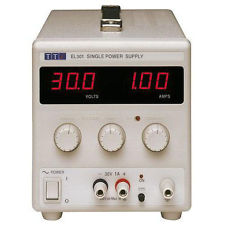
\includegraphics[width=\textwidth]{./images/bench.jpg}
	\caption{A bench power supply}
	\label{fig:benchsupply}
\end{figure}

This device is capable of turning a mains AC supply into a steady DC supply at a set value.
Additionally it has the ability to limit the amount of current that can be drawn.
This is very useful as it makes it harder for you to blow up your circuits.

We will not go into detail about how this works, but basically the three dials allow you to set the voltage and current, then the small switch allows you to switch the output on.
Turn the dials to get $05.0$ shown on the voltage display, and $0.50$ shown on the current display.
This will give us an output of $5V$ with a maximum current draw of $0.5A$.

During use, if the little orange light lights up, please immediately turn the supply output off and ask your supervising blueshirt to have a look.

\subsection{Signal Generators}

\subsection{Multimeters}

\subsection{Breadboard}
The breadboard is a very useful tool, it allows you to construct a circuit quickly and efficiently.
Underneath the plastic cover of the breadboard there are a number of connecting strips.
Along the top and bottom, these strips stretch horizontally halfway across the board, these are often used as the power supplies for the circuit.
In the middle, the strips align vertically connecting up each column of 5 holes.

\subsection{Resistors}
This is a resistor, it is a device used to limit the flow of current.
When a voltage is placed across it a current proportional to the voltage and the resistance of the resistor;

$V = I \times R$

The colour markings on the body of the resistor give the value of the resistor.
On this resistor there are 5 bands in total, the first 4 relate to the value of the resistor, and the final gold band tells us that this is to an accuracy of 5\%.

%%%%%%%%%%%%%%%%%%%%%%%%%%%%%%%%%%%%%%%%%%%%%%%%%%%%%%%%%%%%%%%%%%%%%%%%%%%%%%%%%%%%%%%%%%%%%%%
%V=IR
%
%%%%%%%%%%%%%%%%%%%%%%%%%%%%%%%%%%%%%%%%%%%%%%%%%%%%%%%%%%%%%%%%%%%%%%%%%%%%%%%%%%%%%%%%%%%%%%%

\subsection{Capacitors}


%%%%%%%%%%%%%%%%%%%%%%%%%%%%%%%%%%%%%%%%%%%%%%%%%%%%%%%%%%%%%%%%%%%%%%%%%%%%%%%%%%%%%%%%%%%%%%%
% Q=CV
% Charge over time
% Like fast changes, dislike slow ones
%%%%%%%%%%%%%%%%%%%%%%%%%%%%%%%%%%%%%%%%%%%%%%%%%%%%%%%%%%%%%%%%%%%%%%%%%%%%%%%%%%%%%%%%%%%%%%%

\subsection{Switch}
A switch is like a temporary wire, it creates a connection when the switch is in one position, and breaks the connection when it is in another position.

\subsection{Series}
When devices are connected in series, all the current that flows through one component also flows through the other.

\subsection{Parallel}
Devices that are connected in parallel cause the current to split between them.

It is interesting to note that when resistors are placed in series the resistance is increased, and when they are placed in parallel the resistance decreases.
However when capacitors are placed in series the capacitance is reduced, and when in parallel the capacitance increases.

\subsection{Operational Amplifiers}


%%%%%%%%%%%%%%%%%%%%%%%%%%%%%%%%%%%%%%%%%%%%%%%%%%%%%%%%%%%%%%%%%%%%%%%%%%%%%%%%%%%%%%%%%%%%%%%
% Amplifier
% Output changes proportional to the difference between the two inputs
% 
%%%%%%%%%%%%%%%%%%%%%%%%%%%%%%%%%%%%%%%%%%%%%%%%%%%%%%%%%%%%%%%%%%%%%%%%%%%%%%%%%%%%%%%%%%%%%%%

\subsection{Microcontroller}

The microcontroller is basically the brains of the outfit, it is in essence a mini computer, capable of calculating with a number of different values

%%%%%%%%%%%%%%%%%%%%%%%%%%%%%%%%%%%%%%%%%%%%%%%%%%%%%%%%%%%%%%%%%%%%%%%%%%%%%%%%%%%%%%%%%%%%%%%
%
%%%%%%%%%%%%%%%%%%%%%%%%%%%%%%%%%%%%%%%%%%%%%%%%%%%%%%%%%%%%%%%%%%%%%%%%%%%%%%%%%%%%%%%%%%%%%%%
